\section{Thermodynamic Equilibrium}
\subsection[Thermodynamic Potentials]{Gibbs energy and chemical potential}

\frame{
	\frametitle{Gibbs Energy}
	\begin{itemize}
	\item<1-> Developed  by Josiah Willard Gibbs in 1873.
		\begin{block}{}
		\textit{Available energy} is the greatest amount of mechanical work which can be obtained from a given quantity of a certain substance in a given initial state, without increasing its total volume or allowing heat to pass to or from external bodies, except such as at the close of the processes are left in their initial condition.
		\end{block}
	\item<2-> Relates the \textit{enthalpy} of the system to its \textit{entropy}.
		\begin{exampleblock}{}
		\vspace{-0.25cm}
		\begin{equation*}
		G = H - TS
		\end{equation*}
		\end{exampleblock}
	\item<3-> Gibbs energy is the thermodynamic quantity that is minimised when a system reaches chemical equilibrium at constant temperature and pressure. 
	\end{itemize}
}

\frame{
	\frametitle{Chemical Potential}
	\begin{itemize}
		\item<1-> Chemical potential of species $i$ in phase $\lambda$ is a measure of the change in Gibbs energy of the system by the introduction of species $i$.
		\begin{exampleblock}{}
			\begin{equation*}
        				\mu_{i(\lambda)} = {\left (\frac{\partial G_{sys}}{\partial n_{i(\lambda)}} \right )}_{T,P,n_{j \neq i}}
    			\end{equation*}
		\end{exampleblock}
		
		\item<2-> Ideal mixing phases
		\begin{exampleblock}{}
		\vspace{-0.2cm}
			\begin{equation*}
        				\mu_{i(\lambda)} = g_{i(\lambda)}^0 + \ln x_{i(\lambda)}
    			\end{equation*}
		\end{exampleblock}
		
		\item<3-> Non-ideal mixing phases
		\begin{exampleblock}{}
		\vspace{-0.2cm}
			\begin{equation*}
        				\mu_{i(\lambda)} = g_{i(\lambda)}^0 + \ln x_{i(\lambda)} + g_{i(\lambda)}^{ex}
    			\end{equation*}
		\end{exampleblock}
	\end{itemize}	
}


\frame{
	\frametitle{Gibbs Energy}
	\begin{itemize}
	\item<1-> Integral Gibbs energy of a multicomponent, multiphase system can be expressed in terms of chemical potentials, $\mu_{i(\lambda)}$, of the species.
		\begin{block}{}
		\vspace{-0.15cm}
		\begin{equation*}
        			G_{sys} = RT \left ( \sum_{\lambda=1}^{\Lambda} n_{\lambda} \sum_{i=1}^{N_{\lambda}}x_{i({\lambda})}\tilde{\mu}_i + \sum_{\omega=1}^{\Omega} n_{\omega} \tilde{\mu}_{\omega} \right )
    		\end{equation*}
		\end{block}
	\item<2-> The Gibbs energy of  the system can also be expressed in terms of the element potentials, $\Gamma_j$, and the number of moles, $b_j$, of the system components.
		\begin{exampleblock}{}
		\vspace{-0.15cm}
		\begin{equation*}
		G_{sys} = \sum_{j=1}^{C} \Gamma_j b_j
		\end{equation*}
		\end{exampleblock}
	\end{itemize}
}

\subsection{Conditions of Thermodynamic Equilibrium}
\frame{
	\frametitle{Thermodynamic Equilibrium - Necessary Conditions}
	\pause
	\begin{block}{Conservation of mass}
		\begin{equation*}
		b_j = \sum_{\lambda=1}^{\Lambda} n_{\lambda}\sum_{i=1}^{N_{\lambda}}x_{i({\lambda})}{\nu}_{i,j} +  \sum_{\omega=1}^{\Omega} n_{\omega}{\nu}
		\end{equation*}
	\end{block}
	\pause
	\begin{exampleblock}{Gibbs' phase rule}
		\vspace{-0.1cm}
		\begin{equation*}
		F=C-\Phi + 2 + \Xi
		\end{equation*}
	\end{exampleblock}
	\pause
	\begin{alertblock}{Gibbs' Criteria}
		\begin{equation*}
		\mu_{i} = \sum_{j=1}^C \nu_{i,j} \Gamma_j
		\end{equation*}
	\end{alertblock}		
}

\frame{
	\frametitle{Thermodynamic Equilibrium - Sufficient Conditions}
	\only<1>{
	\begin{block}{Gibbs plane}
	\begin{equation*}
		\pi_{\lambda} = \min_{\lambda} \sum_{i=1}^{N_{\lambda}}x_{i({\lambda})} \left (\mu_{i({\lambda})} - \sum_{j=1}^C \nu_{i,j}\Gamma_j \right )
	\end{equation*}
	\end{block}}
	\only<2>{
	\begin{figure}[htbp]
		\begin{center}
		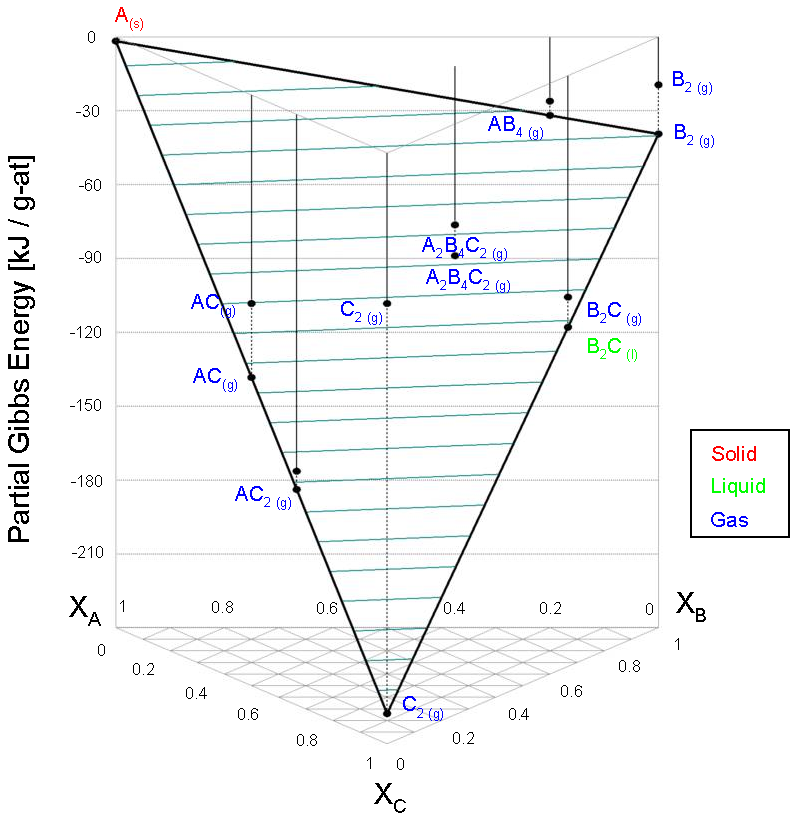
\includegraphics[height=0.75\paperheight]{Figures/Gibbs_plane}
		\end{center}
	\end{figure}
	}
}

\subsection{Gibbs Energy Minimisation}
\frame{
	\frametitle{Gibbs Energy Minimisation}
	\only<1-3>{\begin{itemize}
		\item<1-> Gibbs Energy Minimisation was proposed in 1958 by White, Jonson and Dantzig and is used almost ubiquitously in computation of thermodynamic equilibrium.
		\item<2-> Second order steepest descent method.
		\item<3-> Constrains Gibbs' phase rule while simultaneously minimising the mass balance and Gibbs' criteria residuals.
	\end{itemize}}
	\only<4>{\begin{alertblock}{Optimise}
		\begin{equation*}
		b_j = \sum_{\lambda=1}^{\Lambda} n_{\lambda}\sum_{i=1}^{N_{\lambda}}x_{i({\lambda})}{\nu}_{i,j} +  \sum_{\omega=1}^{\Omega} n_{\omega}{\nu}
		\end{equation*}
	\end{alertblock}
	\begin{exampleblock}{Constraint}
		\vspace{-0.1cm}
		\begin{equation*}
		F=C-\Phi + 2 + \Xi
		\end{equation*}
	\end{exampleblock}
	\pause
	\begin{alertblock}{Optimise}
		\begin{equation*}
		\mu_{i} = \sum_{j=1}^C \nu_{i,j} \Gamma_j
		\end{equation*}
	\end{alertblock}	}
}
